%
% File acl2014.tex
%
% Contact: giovanni.colavizza@epfl.ch
%%
%% Based on the style files for ACL-2013, which were, in turn,
%% Based on the style files for ACL-2012, which were, in turn,
%% based on the style files for ACL-2011, which were, in turn, 
%% based on the style files for ACL-2010, which were, in turn, 
%% based on the style files for ACL-IJCNLP-2009, which were, in turn,
%% based on the style files for EACL-2009 and IJCNLP-2008...

%% Based on the style files for EACL 2006 by 
%%e.agirre@ehu.es or Sergi.Balari@uab.es
%% and that of ACL 08 by Joakim Nivre and Noah Smith

\documentclass[11pt]{article}
\usepackage{acl2014}
\usepackage{times}
\usepackage{url}
\usepackage{latexsym}
\usepackage{graphicx}
\usepackage{subcaption}

%\setlength\titlebox{5cm}

% You can expand the titlebox if you need extra space
% to show all the authors. Please do not make the titlebox
% smaller than 5cm (the original size); we will check this
% in the camera-ready version and ask you to change it back.


\title{How to choose phone's brand according to Amazon}

\author{Marion Kramer\\
  {\tt marion.kramer@epfl.ch} \\\And
  Alexandre Rassinoux \\
  {\tt alexandre.rassinoux@epfl.ch} \\\And
Kristina Satara \\
{\tt kristina.satara@epfl.ch} \\}

\date{18.12.2017}

\begin{document}
\maketitle
\begin{abstract}
 Reviews help when making decision on which product to buy, as they give possible customers personal experiences and more product details. Since customers usually invest some time to study the reviews and ratings before buying specific products from Amazon, the idea of this project is to create evaluation platform which would help the users to choose their future product. For that, insight into  downsides and advantages of various brands based on the reviews will be given. The aim of this project is to analyze reviews of different brands of Amazon cell phone products, and to decide with the help of the reviewms to decide which features are important for specific brands of cell phones. For this natural language processing techniques, such as tf-idf matrix and Latent Dirichlet Allocation will be used.
\end{abstract}


\section{Introduction}
Sentiment analysis, also known as opinion mining or emotion AI, is important part of natural language processing. The subject of the study is the attitude or the emotion behind certain texts. The purpose of sentiment analysis is to determine weather text content is neutral, positive or negative towards some topic. 

Data used for this project is collected from Amazon, during the period of few years. Most of the data is collected between 2012 and 2014, as shown in figure 2. Each of the reviews has also ratings that are used for ground truth. The ratings are based on 5-star system, where 5 is highest and 1 is lowest rating. Distribution of the ratings is J-distribution with highest number of 5-star reviews, and it is shown in figure 1. After purchasing some of the products, customers are asked to give their review and rating, which are further subject to sentiment analysis in our project. Naive Bayes Classifier will be used first, training it with one part of the data, and testing it on the another part. 84\% of correct classifications will be gained when classifying the reviews as positive or negative. After this, bag of words and Latent Dirichlet Allocation (LDA) will be used for extracting interesting features for the brands. 



\begin{figure}[h!]
  \centering
    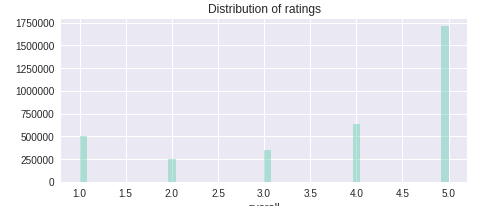
\includegraphics[width=\linewidth]{ratingDistribution.png}
  \caption{Distribution of the ratings in reviews}
  \label{fig:ratingDistribution}
\end{figure}


\begin{figure}[h!]
  \centering
    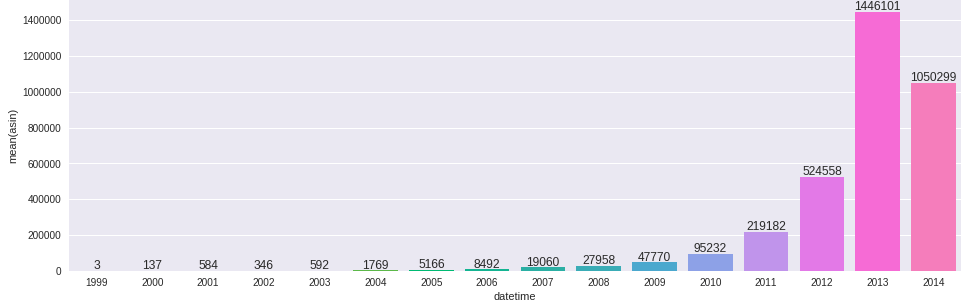
\includegraphics[width=\linewidth]{reviewsByTime.png}
  \caption{Number of reviews during time}
  \label{fig:reviewsByTime}
\end{figure}


\section{Related work}
Natural language processing is an interesting and popular area of research, thus there are many papers regarding this topic. As Amazon is a widely used platform, it has gained much reviews in the past few years. Focus was made on the cell phone reviews, and papers which gave different approaches and conclusions were found. Most of them are using techniques like bag of words and n-grams for sentiment analysis. There is also significant number of papers that are using machine learning techniques for this. Here can be found few examples of papers that are interesting and important regarding this project. In paper "Sentiment Analysis in Amazon Reviews Using Probabilistic Machine Learning" by Callen Rain, the approach is using Naive Bayes Classifier and bigrams for tagging the words for deciding about important features. Another relevant paper in this area of research is "Deep Learning for Amazon Food Review Sentiment Analysis" by Jiayu Wu and Tianshu Ji. They gave diffent approach to the similar problem by using Recurrent Neural Networks for sentiment analysis. 


\section{Data Collection}
The dataset used for this project is provided by Amazon. Dataset consists of two json files - one containing the reviews, and another providing metadata about the products. These two files were merged for further data analysis. The data has also been transformed in order to improve the speed of loading and processing this dataset in the python notebook. As this dataset was incomplete, a decision was made to enrich it with additional dataset from Kaggle platform. This is public GSMArena dataset and it contains more than 8000 phones specifications.


\section{Dataset Description with Summary Statistics}
After merging and combining all the datasets, some descriptive statistics have been made. Given below are the information provided in the datasets:

\begin{itemize}
  \item Reviewer's ID
  \item ID of the product reviewed
  \item Name of the reviewer
  \item Text of the review
  \item Rating given
  \item Summary of the review
  \item Time of the review
  \item Price in euros
  \item Url of the product image
  \item Brand name
  \item Category of the product
\end{itemize}

Firstly, an exploration of the brands of cell phones producers that the dataset contains has been made. As expected, most of the brands are known ones. The interest was given into calculating the mean and median prices of these cell phones. Figure 3. gives overview of mean prices for 25 most popular brands.   

\begin{figure}[h!]
  \centering
    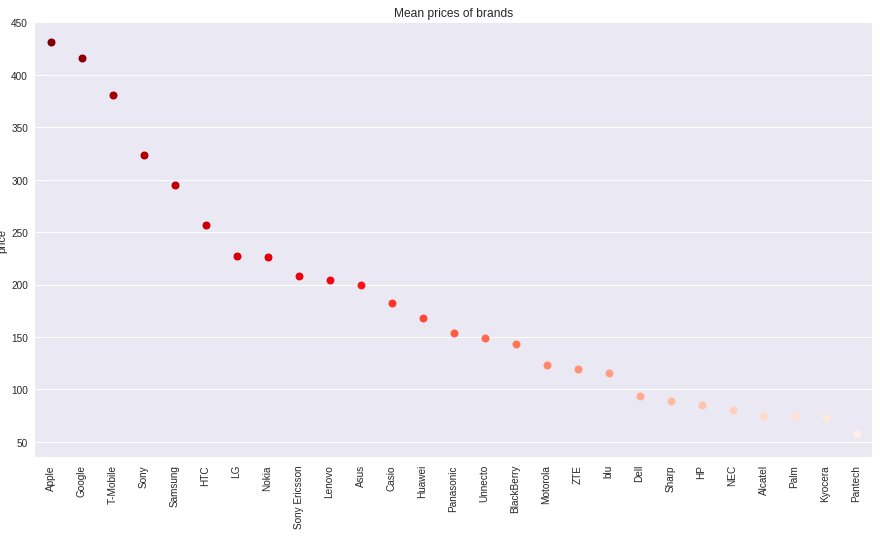
\includegraphics[width=\linewidth]{meanPrices.png}
  \caption{Mean prices per brand}
  \label{fig:meanPricePerBrand}
\end{figure}

Have a look at price distribution can be interesting in order to understand better the dataset and specific models contained in it. It is shown in Figure 4. 

\begin{figure}[h!]
  \centering
    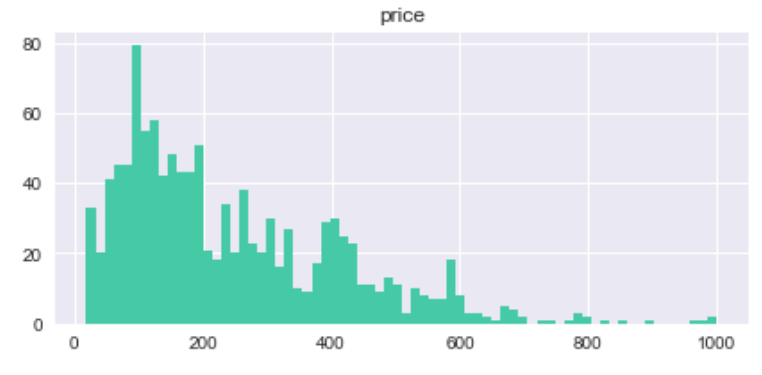
\includegraphics[width=\linewidth]{priceDistribution.png}
  \caption{Distribution of the prices}
  \label{fig:priceDistribution}
\end{figure}

Another statistics that is interesting is average number of cell phone models per brand, mean ratings per brand, and models that have highest number of the reviews. 

Customer's decision about purchasing specific model is often influenced by overall rating of the product - but in the project it has been shown that this rating should be taken very carefully when used for making decisions. This is not the rating of specific model that is important, but also the number of reviews. During the exploratory analysis, it was found that some models only have a few reviews, but their rating is the highest possible, and there are other models that have an average rating above four and also have few thousand times more reviews. This should be taken into consideration very carefully before the decision. \par\par

There are no correlations between the price and the rating. Figure 5. shows example of correlation of words with the ratings - either high or low rating for specific brand, in this case it is Sony Ericsson. It can be seen that some words have higher correlation with the reviews - for example battery and phone. 


\begin{figure}[h!]
  \centering
    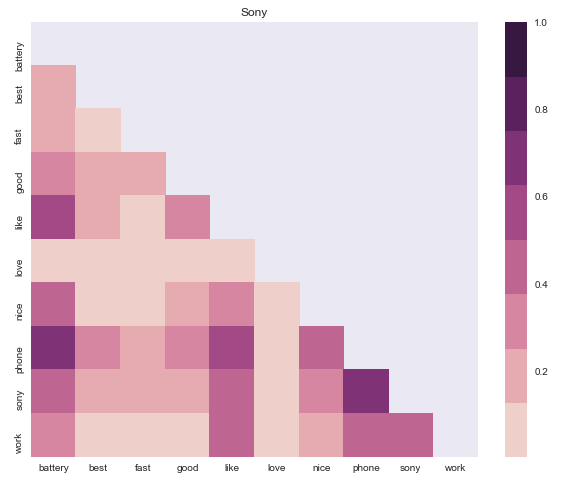
\includegraphics[width=\linewidth]{correlations.png}
  \caption{Correlations of the words with reviews}
  \label{fig:correlations}
\end{figure}

This was the basic analysis of the dataset. Further analysis is closely connected to the natural language processing and sentiment analysis, thus it will be explained into more details in the next section. 


\section{Methods}
Two approaches were used in order to find the important features of cell phone brands. The first approach is to use supervised learning to classify new review as positive or negative. After this, extraction of important words was made and a sentiment analysis for the review using bag of words approach and Latent Dirichlet Allocation was done.


\subsection{Naive Bayes Classifier}

The reviews are split into positive and negative based on the ratings, and they are separately analysed. Decision was made that ratings four and five will be positive reviews, and one and two will be negative reviews. Reviews rated with three were not taken into account because they were considered as neutral reviews. After marking the reviews as positive, negative, or neutral, supervised learning was used to check if it was possible to train the model to predict if some new review is positive or negative. The reviews are first tokenized, and stopwords are removed. After this, lemmatization is done in order to merge the different forms of the same word into one, by removing affixes. \par


90\% of the data were used for training and 10\% for the validation, and with Naive Bayes Classifier, result of ~84\% of successful classification was obtained. Most important features for classifying the review as negative are words scam and false, whereas for classifying the review as positive important words are perfect and excellent. As the aim of this project is not to find only the important features, but to determine which of some specific features - like battery, ergonomy, screen, camera, etc - are correlated and important for some brands, a second step of analysis is needed to go futher in the analysis.


\subsection{Further sentiment analysis} 

Here a sligthly modified approach was used. The next steps were made: 

 \begin{itemize}
  \item First the reviews were split according to the brand and according to the ratings - five groups are created for ratings from one to five.
  \item Next topic modelling is done using words vectors and Latent Dirichlet Allocation (LDA). Reviews are seen as a bag of words, and topics as a distribution over a fixed vocabulary. Words are generated from document specific topic distributions. As the output of this step, 10 topics with the 10 most important words for each topic (for each brand) have been found.
  \item After this, a sentiment is tagged on topic words. The previous Sentiment Analyzer has been used in order to get a weighted sentiment for the topic. Here two kind of words have been considered. First are feature words that are where the most interest is - like battery or screen. Second group of words are non-feature words (great, bad, problem, work, etc). Non-feature words in the topic will be subject to sentiment analysis. 
  \item The weighted scores of all the non-feature words will be given to all the feature words in the following topic. If a topic does not contain feature words, it is ignored.
  \item At the end, the results are groupped to get an overview for all the reviews and all ratings. The density of appearence for each feature word in each topic is counted. As a result, the sum of polarity scores for each feature word is shown.
\end{itemize}


\section{Results and Findings}
From the exploratory analysis the next conclusions can be made: The years when there were the higher number of reviews are 2013. and 2014. Overall the most reviewed models by the customers are Samsung Galaxy S3 Mini, Nokia N8, Motorola Moto G. Best rated cell phones are not always the best choise, as they sometimes have only few reviews. There are no correlations of the prices and ratings. Based on our dataset, the higher mean price of cell phones has Apple with average price of almost 450 euros. 
 \par

Regarding the sentiment analysis, for each brand there are usually more positive than negative reviews. As explained in the previous part, using the bag of words and Latent Dirichlet Allocation and analysing the important feature words, the results obtained are shown on the Figure 6.  TODO: ALEX INSERT THE NICE FIGURE HERE AND ADD FEW SENTENCES HERE TO CONCLUDE PLEASE :)

\section{Conclusion}
This platform uses reviews and extracts meaningful information from it, and then evaluates certain cell phone brand based on these reviews. Sentiment analysis was used to classify each of the reviews and it's parts as good or bad. After this process, appeareances and sentiments have been found for the feature words (for example battery, screen, camera, etc). For the review preprocessing, the next techniques are used : tokenization, removal of the stopwords, lemmatization. \par

For classifying the reviews, Naive Bayes Classifier is used, while for detecting the feature words, bag of words and Latent Dirichlet Allocation were used. Based on this, specific brands and features that customers find important for certain cell phone brands are described and evaluated.  

\begin{thebibliography}{}

\bibitem[\protect\citename{wallin}]{Aho:72}
Alexander Wallin.
\newblock {\em Sentiment analysis of Amazon reviews and perception of product features}.


\bibitem[\protect\citename{Liu-Bing}]{Aho:72}
Bing Liu.
\newblock {\em Sentiment Analysis and Opinion Mining}.
\newblock Synthesis Lectures on Human Language Technologies.


\bibitem[\protect\citename{Callen Rain}]{Aho:72}
Callen Rain.
\newblock {\em Sentiment Analysis in Amazon Reviews Using Probabilistic Machine Learning }.
\newblock Swarthmore College.


\bibitem[\protect\citename{Elli-Wang}]{Aho:72}
Maria Soledad Elli, Yi-Fan Wang.
\newblock {\em Amazon Reviews, business analytics with sentiment analysis}.
\newblock Department of Computer Science, North Carolina A\&T State University, USA.


\bibitem[\protect\citename{Fang Zhan}]{Aho:72}
Xing Fang and Justin Zhan.
\newblock 2015.
\newblock { \em Sentiment analysis using product review data }.
\newblock Department of Computer Science, North Carolina A\&T State University, USA.



\end{thebibliography}

\end{document}
